
\subsection{Meshes}

Describe meshes and material properties used for testing.

\begin{figure}
	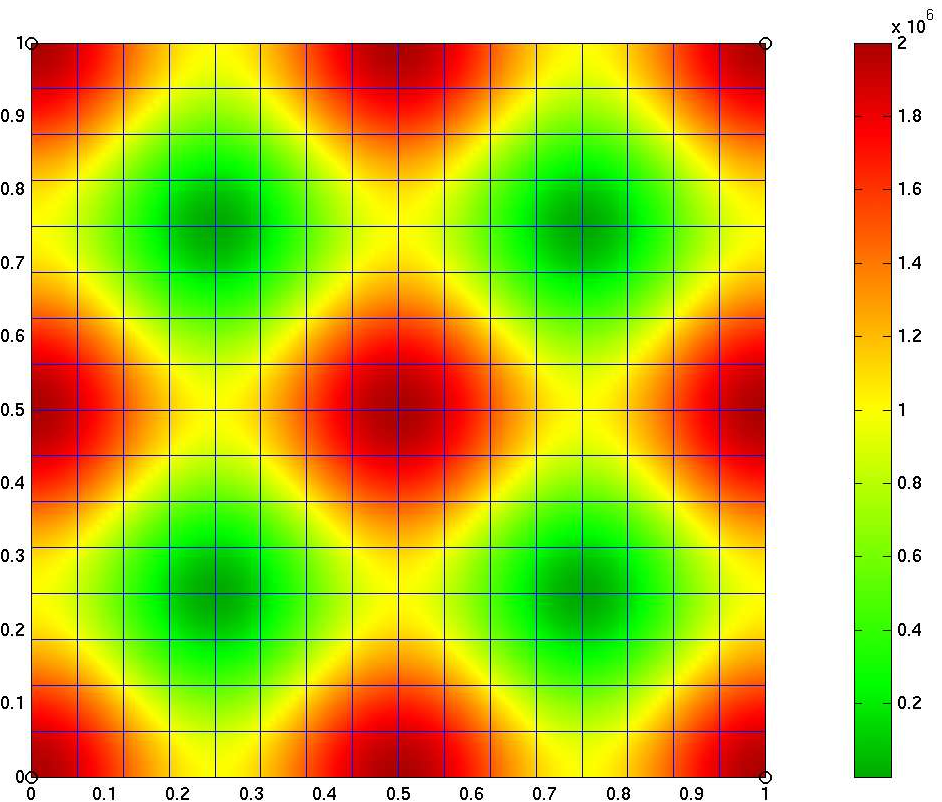
\includegraphics[width=0.45\textwidth]{figs/box}
	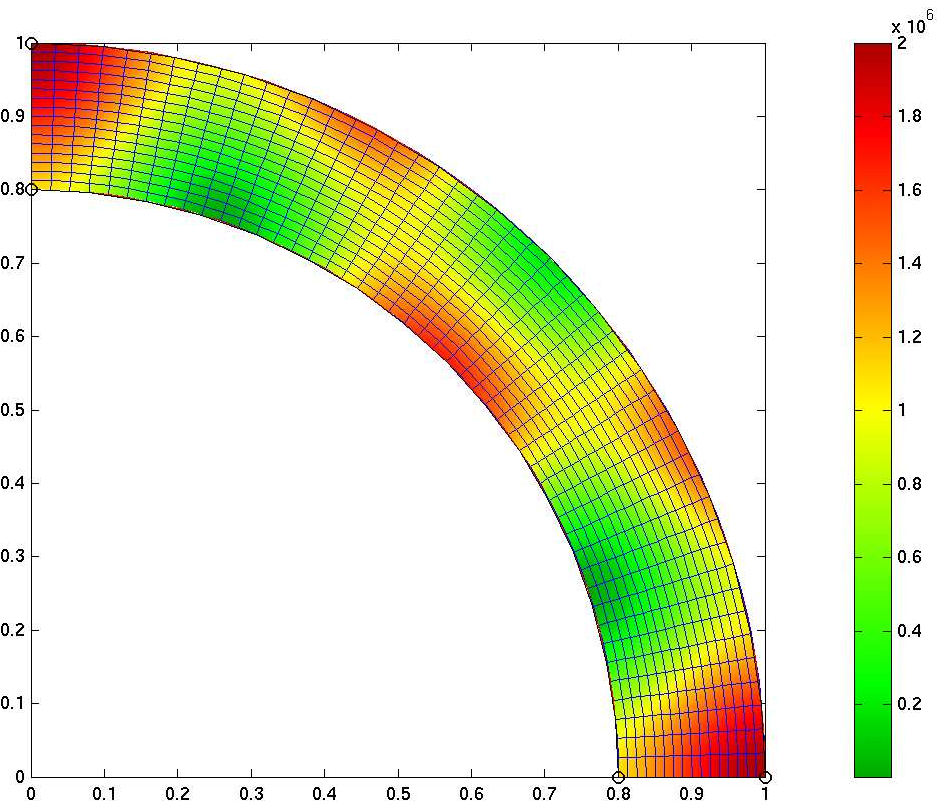
\includegraphics[width=0.45\textwidth]{figs/fan}
	\caption{\label{fig:mesh2d} The 2D meshes used for the tests.}
\end{figure}

\begin{figure}
	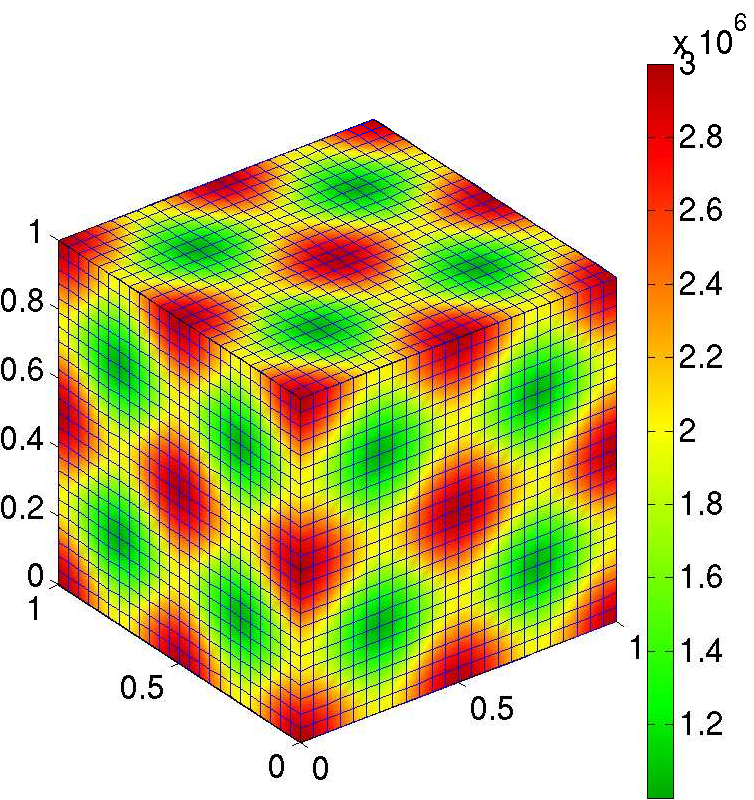
\includegraphics[width=0.45\textwidth]{figs/box3a}
	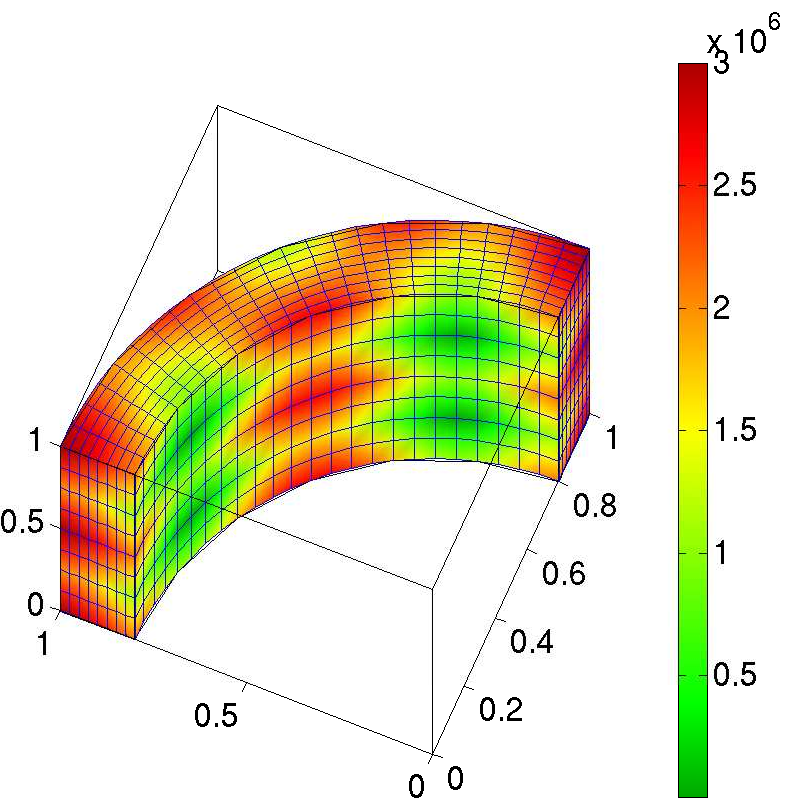
\includegraphics[width=0.45\textwidth]{figs/fan3a}
	\caption{\label{fig:mesh3d} The 3D meshes used for the tests.}
\end{figure}


\begin{table}
  \caption{\label{tab:box} Number of CG iterations/v-cycles to converge to a relative tolerance of $10^{-8}$ for $h$-Multigrid applied to high-order operators on a rectangular domain. A total of 3 grids were used, the finest grid was $32\times 32$, and the coarsest was $8\times 8$. For orders $2,4$, and $8$, we also evaluated the option of first coarsening in $p$ as $p_{coarse} = p_{fine}/2$, till $p=1$, and then coarsen in $h$. The coarsest grid in this case is a $8\times 8$ grid with $p=1$. The number of CG iterations/v-cycles for this case is given in the $p$ column.}
		\centering
    \begin{tabular}{|l|c|c|c|c|c|c|c|c|c|c|c|c|r|} 
\hline
                     & \multicolumn{6}{c|}{Multigrid} & \multicolumn{6}{c|}{MG pCG} &          linearized \\
										 \cline{2-13}
			order &  \multicolumn{2}{c|}{\scriptsize  Jacobi(3)} &  \multicolumn{2}{c|}{\scriptsize Chebyshev(3)} & \multicolumn{2}{c|}{\scriptsize  SSOR(2)} & \multicolumn{2}{c|}{\scriptsize Jacobi(3)} &  \multicolumn{2}{c|}{\scriptsize Chebyshev(3)} & \multicolumn{2}{c|}{\scriptsize SSOR(2)} & pCG\\
\hline
 & $h$ & $p$ & $h$ & $p$& $h$ & $p$& $h$ & $p$& $h$ & $p$& $h$ & $p$& \\
 \cline{2-13}
                   1 &       6 &    &                         5 &    &                 4 &   &                    4 &     &                      4 &      &               4 &   &    4\\
                   2 &   7     & 7  &                         9 & 9  &                 4 & 4 &                    5 &  5  &                      6 &  6   &               4 & 4 &   14\\
                   3 &       8 &    &                        22 &    &                 5 &   &                    6 &     &                     10 &      &               4 &   &   21\\
                   4 &       - & -  &                        48 & 46 &                 8 & 7 &                   43 & 39  &                     15 &  15  &               6 & 5 &   30\\
                   5 &       - &    &                       150 &    &                12 &   &                  295 &     &                     27 &      &               8 &   &   43\\
                   6 &       - &    &                         - &    &                27 &   &                    - &     &                     51 &      &              12 &   &   65\\
                   7 &       - &    &                         - &    &                81 &   &                    - &     &                    105 &      &              21 &   &   99\\
                   8 &       - & -  &                         - & -  &                298&267&                    - &  -  &                    204 &  182 &              39 &36 &  146\\
\hline
	  \end{tabular}
\end{table}

% \begin{table}
%   \caption{\label{tab:hpmg} Number of CG iterations/v-cycles to converge to a relative tolerance of $10^{-8}$ for $hp$-Multigrid applied to high-order operators on a rectangular domain. Starting with a $32\times 32$ high-order grid, we first coarsen in $p$ till $p=1$, and then coarsen in $h$. The coarsest grid in all cases is a $8\times 8$ grid with $p=1$}
% 		\centering
% 		\begin{tabular}{|l|c|c|c|c|c|c|} 
% 	    \hline
% 				    & \multicolumn{3}{c|}{Multigrid} & \multicolumn{3}{c|}{MG pCG}\\  \cline{2-7}
% 			order & \scriptsize Jacobi(3)  &\scriptsize  Chebyshev(3)  &\scriptsize SSOR(2) &\scriptsize Jacobi(3)  &\scriptsize  Chebyshev(3)  &\scriptsize SSOR(2) \\
% 			\hline
% 				1 & 6  &  5 &  4 & 4 & 4 & 4 \\ 
% 	    	2 & 7 & 9  & 4 & 5 & 6 & 4 \\
% 				%3 & 8 & 24 & 5 & 6 & 11 & 4 \\
% 				4 & - & 46 & 7 & 39 & 15 & 5 \\
% 				%5 & - & 178 & 13 & - & 28 & 8 \\
% 				%6 & - & - & 24 & - & 51 & 12 \\
% 				%7 & - & - & 70 & - & 105 & 19 \\
% 				8 & - & - & 267 & - & 182 & 36 \\
% 			\hline
% 	  \end{tabular}
% \end{table}


\begin{table}
  \caption{\label{tab:fan} Number of CG iterations/v-cycles to converge to a relative tolerance of $10^{-8}$ for $h$-Multigrid applied to high-order operators on a fan domain. A total of 3 grids were used, the finest grid was $48\times 16$, and the coarsest was $12\times 4$. For orders $2,4$, and $8$, we also evaluated the option of first coarsening in $p$ as $p_{coarse} = p_{fine}/2$, till $p=1$, and then coarsen in $h$. The coarsest grid in this case is a $12\times 4$ grid with $p=1$. The number of CG iterations/v-cycles for this case is given in the $p$ column.}
		\centering
    \begin{tabular}{|l|c|c|c|c|c|c|c|c|c|c|c|c|r|} 
\hline
		 & \multicolumn{6}{c|}{Multigrid} & \multicolumn{6}{c|}{MG pCG} &          linearized \\
		\cline{2-13}
		order &  \multicolumn{2}{c|}{\scriptsize  Jacobi(3)} &  \multicolumn{2}{c|}{\scriptsize Chebyshev(3)} & \multicolumn{2}{c|}{\scriptsize  SSOR(2)} & \multicolumn{2}{c|}{\scriptsize Jacobi(3)} &  \multicolumn{2}{c|}{\scriptsize Chebyshev(3)} & \multicolumn{2}{c|}{\scriptsize SSOR(2)} & pCG\\
				 \hline
				  & $h$ & $p$ & $h$ & $p$& $h$ & $p$& $h$ & $p$& $h$ & $p$& $h$ & $p$& \\
				  \cline{2-13}
         
 1 &       7 &       &         8 &       &       4 &       &         5 &        &         6 &      &             4 &     &  4  \\
 2 &       9 &   9   &        12 &  13   &       5 &   5   &         6 &   6    &         7 &  8   &             4 &  4  &  55  \\
 3 &      10 &       &        26 &       &       5 &       &         7 &        &        12 &      &             4 &     &  129  \\
 4 &       - &   -   &        54 &  55   &       8 &   7   &       136 &  79    &        17 & 17   &             6 &  6  &  235  \\
 5 &       - &       &       171 &       &      14 &       &         - &        &        31 &      &             8 &     &  430  \\
 6 &       - &       &         - &       &      42 &       &         - &        &        53 &      &            15 &     &  663  \\
 7 &       - &       &         - &       &     146 &       &         - &        &       109 &      &            29 &     &  804  \\
 8 &       - &       &         - &   -   &       - &   -   &         - &   -    &        -  & 270  &            85 & 70  &  1015  \\
\hline
	  \end{tabular}
\end{table}


% \begin{table}
%   \caption{\label{tab:hpmg} Number of CG iterations/v-cycles to converge to a relative tolerance of $10^{-8}$ for $hp$-Multigrid applied to high-order operators on a stretched fan domain. Starting with a $48\times 16$ high-order grid, we first coarsen in $p$ till $p=1$, and then coarsen in $h$. The coarsest grid in all cases is a $12\times 4$ grid with $p=1$}
% 		\centering
% 		\begin{tabular}{|l|c|c|c|c|c|c|} 
% 	    \hline
% 				    & \multicolumn{3}{c|}{Multigrid} & \multicolumn{3}{c|}{MG pCG}\\  \cline{2-7}
% 			order & \scriptsize Jacobi(3)  &\scriptsize  Chebyshev(3)  &\scriptsize SSOR(2) &\scriptsize Jacobi(3)  &\scriptsize  Chebyshev(3)  &\scriptsize SSOR(2) \\
% 			\hline
% 				1 & 7  &  8 &  4 & 5 & 6 & 4 \\ 
%         2 & 9 & 13 & 5 & 6 & 8 & 4 \\
% 				4 & - & 55 & 7 & 79 & 17 & 6 \\
%         8 & - & - & - & - & 270 & 70 \\
% 			\hline
% 	  \end{tabular}
% \end{table}

%% anisotropy - stretched fan
\begin{table}
  \caption{\label{tab:fan-aniso} Number of CG iterations/v-cycles to converge to a relative tolerance of $10^{-8}$ for $h$-Multigrid applied to high-order operators on a stretched fan domain. A total of 3 grids were used, the finest grid was $48\times 16$, and the coarsest was $12\times 4$. For orders $2,4$, and $8$, we also evaluated the option of first coarsening in $p$ as $p_{coarse} = p_{fine}/2$, till $p=1$, and then coarsen in $h$. The coarsest grid in this case is a $12\times 4$ grid with $p=1$. The number of CG iterations/v-cycles for this case is given in the $p$ column.}
		\centering
    \begin{tabular}{|l|c|c|c|c|c|c|c|c|c|c|c|c|r|} 
\hline
		        & \multicolumn{6}{c|}{Multigrid} & \multicolumn{6}{c|}{MG pCG} &          linearized \\
												 \cline{2-13}
					order &  \multicolumn{2}{c|}{\scriptsize  Jacobi(3)} &  \multicolumn{2}{c|}{\scriptsize Chebyshev(3)} & \multicolumn{2}{c|}{\scriptsize  SSOR(2)} & \multicolumn{2}{c|}{\scriptsize Jacobi(3)} &  \multicolumn{2}{c|}{\scriptsize Chebyshev(3)} & \multicolumn{2}{c|}{\scriptsize SSOR(2)} & pCG\\
		\hline
		 & $h$ & $p$ & $h$ & $p$& $h$ & $p$& $h$ & $p$& $h$ & $p$& $h$ & $p$& \\
		 \cline{2-13}
 1 &       16 &      &        21 &        &       6 &         &       9 &         &       10 &       &       5 &      & 5  \\
 2 &       22 &  23  &        24 &  24    &       7 &   7     &      10 &  11     &       11 &  11   &       5 &   5  & 67  \\
 3 &        - &      &        54 &        &       8 &         &      55 &         &       17 &       &       6 &      & 160  \\
 4 &        - &  -   &        97 &  92    &      14 &   13    &       - &         &       23 &  22   &       9 &   8  & 262  \\
 5 &        - &      &       313 &        &      22 &         &       - &         &       41 &       &      11 &      & 444  \\
 6 &        - &      &         - &        &      76 &         &       - &         &       73 &       &      21 &      & 654  \\
 7 &        - &      &         - &        &     259 &         &       - &         &      161 &       &      38 &      & 941  \\
 8 &        - &  -   &         - &  -     &       - &    -    &       - &         &        - & 271   &      88 &  72  & 1150  \\
\hline
	  \end{tabular}
\end{table}


% \begin{table}
%   \caption{\label{tab:hpmg} Number of CG iterations/v-cycles to converge to a relative tolerance of $10^{-8}$ for $hp$-Multigrid applied to high-order operators on a fan domain. Starting with a $48\times 16$ high-order grid, we first coarsen in $p$ till $p=1$, and then coarsen in $h$. The coarsest grid in all cases is a $12\times 4$ grid with $p=1$}
% 		\centering
% 		\begin{tabular}{|l|c|c|c|c|c|c|} 
% 	    \hline
% 				    & \multicolumn{3}{c|}{Multigrid} & \multicolumn{3}{c|}{MG pCG}\\  \cline{2-7}
% 			order & \scriptsize Jacobi(3)  &\scriptsize  Chebyshev(3)  &\scriptsize SSOR(2) &\scriptsize Jacobi(3)  &\scriptsize  Chebyshev(3)  &\scriptsize SSOR(2) \\
% 			\hline
% 				1 & 6  &  5 &  4 & 4 & 4 & 4 \\ 
%         2 & 9 & 12 & 5 & 6 & 8 & 4 \\
% 				4 & - & 53 & 7 & 100 & 16 & 6 \\
%         8 & - & -  & - & - & 200 & 60 \\
% 			\hline
% 	  \end{tabular}
% \end{table}


%% 3D

\begin{table}
  \caption{\label{tab:box3} Number of CG iterations/v-cycles to converge to a relative tolerance of $10^{-8}$ for $h$-Multigrid applied to high-order operators on a cube domain. A total of 3 grids were used, the finest grid was $8\times 8\times 8$, and the coarsest was $2\times 2\times 2$. For orders $2,4$, and $8$, we also evaluated the option of first coarsening in $p$ as $p_{coarse} = p_{fine}/2$, till $p=1$, and then coarsen in $h$. The coarsest grid in this case is a $2\times 2\times 2$ grid with $p=1$. The number of CG iterations/v-cycles for this case is given in the $p$ column.}
		\centering
    \begin{tabular}{|l|c|c|c|c|c|c|c|c|c|c|c|c|r|} 
	    \hline
						        & \multicolumn{6}{c|}{Multigrid} & \multicolumn{6}{c|}{MG pCG} &          linearized \\
																 \cline{2-13}
									order &  \multicolumn{2}{c|}{\scriptsize  Jacobi(3)} &  \multicolumn{2}{c|}{\scriptsize Chebyshev(3)} & \multicolumn{2}{c|}{\scriptsize  SSOR(2)} & \multicolumn{2}{c|}{\scriptsize Jacobi(3)} &  \multicolumn{2}{c|}{\scriptsize Chebyshev(3)} & \multicolumn{2}{c|}{\scriptsize SSOR(2)} & pCG\\
						\hline
						 & $h$ & $p$ & $h$ & $p$& $h$ & $p$& $h$ & $p$& $h$ & $p$& $h$ & $p$& \\
						 \cline{2-13}
						 
1 & 7  &  7  & 15  & 15  &  5   &  5   & 5    &  5   &  8   &   8    & 4   &  4   & 4    \\
2 & 8  &  8  & 43  & 50  &  4   &  5   & 6    &  6   &  15  &  15    & 4   &  4   & 25   \\
3 & 10 &     & 141 &     &  5   &      & 7    &      &  27  &        & 4   &      & 45   \\
4 & -  &  -  & -   &  -  &  10  &  9   & 111  &  85  &  50  &  47    & 7   &  6   & 79   \\
5 & -  &     & -   &     &  19  &      & -    &      &  102 &        & 10  &      & 144  \\
6 & -  &     & -   &     &  56  &      & -    &      &  234 &        & 18  &      & 260  \\
7 & -  &     & -   &     &  250 &      & -    &      &  -   &        & 37  &      & 465  \\	
8 & -  &  -  & -   &  -  &  -   &  -   & -    &   -  &  -   &   -    & 96  & 90   & 840  \\
			\hline
	  \end{tabular}
\end{table}

% \begin{table}
%   \caption{\label{tab:box3p} Number of CG iterations/v-cycles to converge to a relative tolerance of $10^{-8}$ for $hp$-Multigrid applied to high-order operators on a cube domain. Starting with a $8\times 8\times 8$ high-order grid, we first coarsen in $p$ till $p=1$, and then coarsen in $h$. The coarsest grid in all cases is a $2\times 2\times 2$ grid with $p=1$}
% 		\centering
% 		\begin{tabular}{|l|c|c|c|c|c|c|} 
% 	    \hline
% 				    & \multicolumn{3}{c|}{Multigrid} & \multicolumn{3}{c|}{MG pCG}\\  \cline{2-7}
% 			order & \scriptsize Jacobi(3)  &\scriptsize  Chebyshev(3)  &\scriptsize SSOR(2) &\scriptsize Jacobi(3)  &\scriptsize  Chebyshev(3)  &\scriptsize SSOR(2) \\
% 			\hline
%         1 & 7 & 15 & 5 & 5 & 8 & 4 \\
%         2 & 8 & 50 & 5 & 6 & 15 & 4 \\
% 			  4 & - & - & 9 & 85 & 47 & 6 \\
%         8 & - & - & - & -  &  - & 90 \\
%       \hline
% 	  \end{tabular}
% \end{table}

\begin{table}
  \caption{\label{tab:fan3} Number of CG iterations/v-cycles to converge to a relative tolerance of $10^{-8}$ for $h$-Multigrid applied to high-order operators on a 3d fan domain. A total of 3 grids were used, the finest grid was $12\times 4\times 4$, and the coarsest was $6\times 2\times 2$.}
		\centering
    \begin{tabular}{|l|c|c|c|c|c|c|c|c|c|c|c|c|r|} 
	    \hline
						        & \multicolumn{6}{c|}{Multigrid} & \multicolumn{6}{c|}{MG pCG} &          linearized \\
																 \cline{2-13}
									order &  \multicolumn{2}{c|}{\scriptsize  Jacobi(3)} &  \multicolumn{2}{c|}{\scriptsize Chebyshev(3)} & \multicolumn{2}{c|}{\scriptsize  SSOR(2)} & \multicolumn{2}{c|}{\scriptsize Jacobi(3)} &  \multicolumn{2}{c|}{\scriptsize Chebyshev(3)} & \multicolumn{2}{c|}{\scriptsize SSOR(2)} & pCG\\
						\hline
						 & $h$ & $p$ & $h$ & $p$& $h$ & $p$& $h$ & $p$& $h$ & $p$& $h$ & $p$& \\
						 \cline{2-13}
						 
1 &  17  & 17 &  35  & 35  & 7   &  7  & 8   &  8  & 13  & 13  & 5  &  5   &   5 \\
2 &  23  & 25 &  69  & 78  & 8   &  9  & 11  &  11 & 19  & 20  & 6  &  6   &  45 \\  
3 &  -   &    &  158 &     & 12  &     & 136 &     & 30  &     & 7  &      &  97 \\
4 &  -   & -  &   -  &  -  & 25  & 21  &  -  &  -  & 54  & 56  & 11 & 10   & 204 \\
5 &  -   &    &   -  &     & 33  &     &  -  &     & 118 &     & 14 &      & 451 \\ 
6 &  -   &    &   -  &     & XX  &     &  -  &     & XX  &     & XX &      & 915 \\ 
7 &  -   &    &   -  &     & XX  &     &  -  &     &  -  &     & XX &      & 1000+ \\ 
8 &  -   &    &   -  &     & XX  &     &  -  &     &  -  &  -  & XX &  XX  & 1000+ \\ 
			\hline
	  \end{tabular}
\end{table}
% 
% \begin{table}
%   \caption{\label{tab:fan3p} Number of CG iterations/v-cycles to converge to a relative tolerance of $10^{-8}$ for $hp$-Multigrid applied to high-order operators on a 3d fan domain. Starting with a $8\times 8\times 8$ high-order grid, we first coarsen in $p$ till $p=1$, and then coarsen in $h$. The coarsest grid in all cases is a $2\times 2\times 2$ grid with $p=1$}
% 		\centering
% 		\begin{tabular}{|l|c|c|c|c|c|c|} 
% 	    \hline
% 				    & \multicolumn{3}{c|}{Multigrid} & \multicolumn{3}{c|}{MG pCG}\\  \cline{2-7}
% 			order & \scriptsize Jacobi(3)  &\scriptsize  Chebyshev(3)  &\scriptsize SSOR(2) &\scriptsize Jacobi(3)  &\scriptsize  Chebyshev(3)  &\scriptsize SSOR(2) \\
% 			\hline
%         1 & 17 & 35 & 7 & 8 & 13 & 5 \\
%         2 & 25 & 78 & 9 & 11 & 20 & 6 \\
%         4 & - & - & 21 & - & 56 & 10 \\
%       \hline
% 	  \end{tabular}
% \end{table}
